\newpage
\hypertarget{treeToModel tex}{}
\subsection{Tree To model text source}
\texHeader

\begin{itemize}

\item[$\blacktriangleright$] So we've already established one schema. Plan : separate the transformation into smaller, modular steps. First: Transform the
parent folder into a library. Then we want to establish every subfolder as a shelf  (i.e., english and french) We then want to take each dictionary file in
those folders, and turn them into dictionary objects with a defined author and set of entries.

\item[$\blacktriangleright$] Right-click on ``Rules/New TGG Rule" and create \texttt{FolderToLibrayRule}.

\item[$\blacktriangleright$] This is a simple rule - all we need to do is create a folder and library object, create a link between them ( so that we're
always within their context) and create a constraint equating the name of the folder to the name of the library. Build your rule until it resembles FIG
(remember: target is MOCATREE, source is DICTIONARYLANGUAGE)

\begin{figure}[htbp]
\begin{center}
  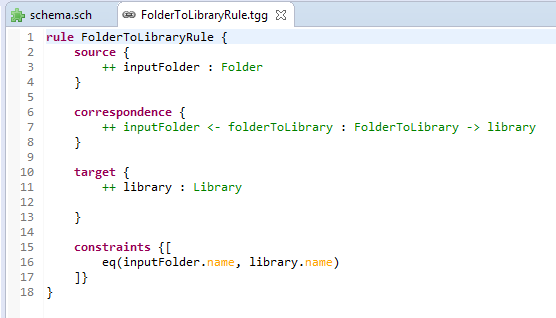
\includegraphics[width=\textwidth]{eclipse_FolderToLibraryRule}
  \caption{Folder to Library Rule complete}
  \label{eclipse:FolderToLibraryRule}
\end{center}
\end{figure}

\item[$\blacktriangleright$] Now we want \texttt{ForAllShelves}. A driving reason why this rule is independent and not included with \texttt{FolderToLibrary} is
because we simply don't know how many subfolders the original library folder will have. This rule will invoked whenever there is the context of an input folder
and library already made. Build it until it resembles FIG

\begin{figure}[htbp]
\begin{center}
  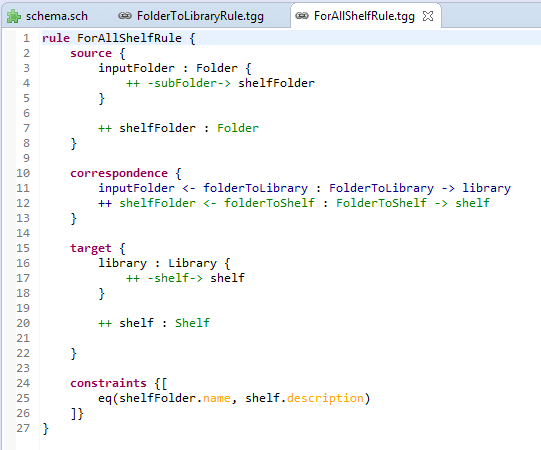
\includegraphics[width=\textwidth]{eclipse_ForAllShelfRule}
  \caption{ForAllShelves complete}
  \label{eclipse:ForAllShelvesRule}
\end{center}
\end{figure}

\item[$\blacktriangleright$] Don't forget to update the schema with your newest correspondence! When you saved, you should have received an error about it.

\item[$\blacktriangleright$] Next, the third major part of our transformation: the dictionary files into the dictionary tree. If you look at the
\texttt{tree.xmi}, you'll notice that each \texttt{.dictioanry} file is turned into a dictionary \texttt{Node} with at least three children - one node for the
title of the dictionary, one for the email address of the author, and one node per entry object. We know we'll always have a title, but we'll never know if an
author will be included, or how many entries. We'll need to keep these separate. therefore, This step will actually require \emph{at least} three rules. Lets
build the biggest one first, the primary \texttt{NodeToDictionaryRule}. Build it as depicted below.

\item[$\blacktriangleright$] Think: what do we already know from the context?? You'll notice from \texttt{tree.xmi} that the title, author, and entry nodes each
ahve different indexes in order to tell them apart. So, lets bind index0 to title node to guarantee we'll get the right info

\begin{figure}[htbp]
\begin{center}
  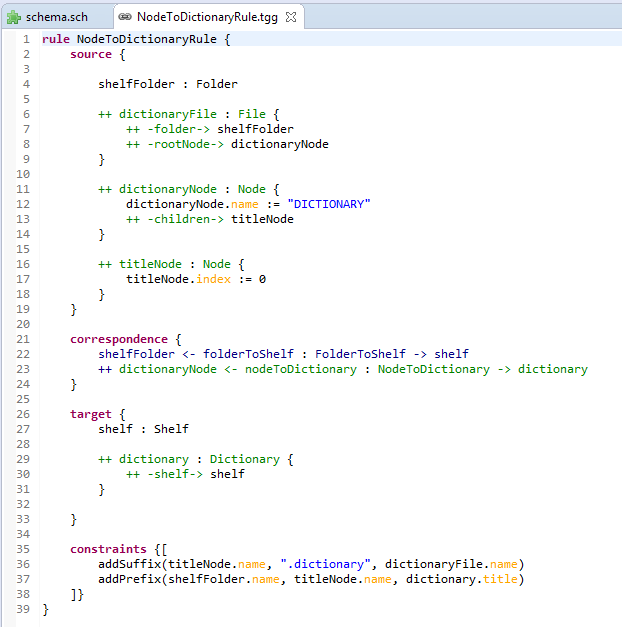
\includegraphics[width=\textwidth]{eclipse_NodeToDictionaryRule}
  \caption{NodeToDictionary complete}
  \label{eclipse:NodeToDictionaryRule}
\end{center}
\end{figure}

\item[$\blacktriangleright$] Now we have to deal with authors and entries. Let's build entries first.

\begin{figure}[htbp]
\begin{center}
  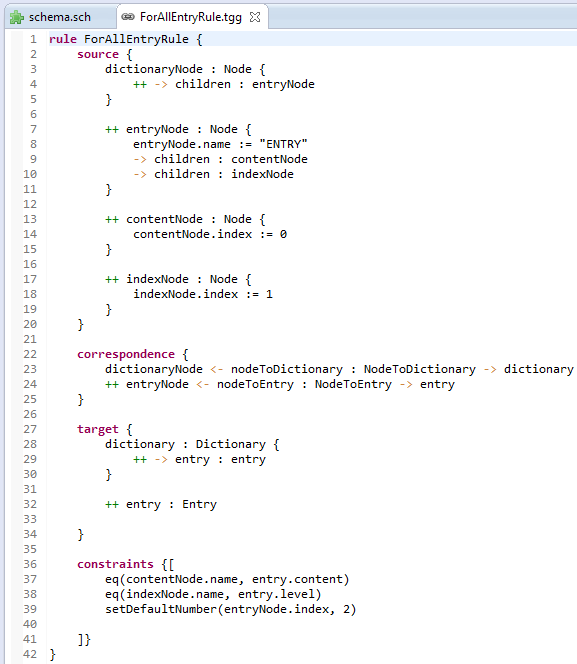
\includegraphics[width=\textwidth]{eclipse_ForAllEntryRule}
  \caption{NodeToDictionary complete}
  \label{eclipse:NodeToDictionaryRule}
\end{center}
\end{figure}

\item[$\blacktriangleright$] Now the challenge of an author. You'll notice we have three parts to this challenge: \texttt{unknown.dictioanry} doesn't even have
one, so that means we'll definitely need to have it separated from \texttt{NodeToDictionary}. Then, we need to be able to provide the option of creating or
ignoring a new author element in a library if one already existts (try and motivate better\ldots)

\item[$\blacktriangleright$] Lets create \texttt{ForAllNewAuthorRule} first

\begin{figure}[htbp]
\begin{center}
  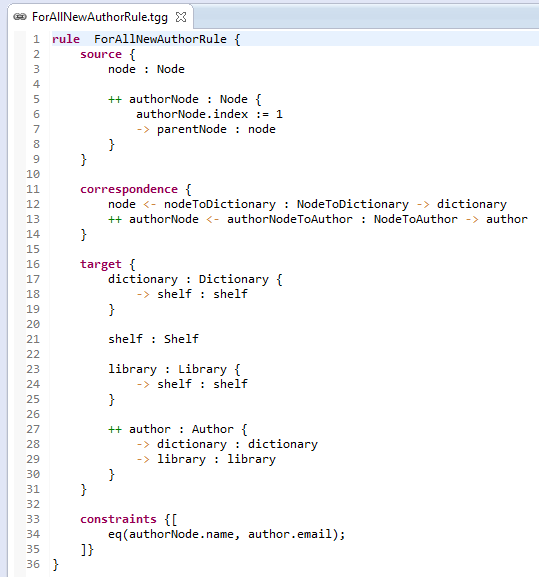
\includegraphics[width=\textwidth]{eclipse_ForAllNewAuthorRule}
  \caption{ForAllAuthor complete}
  \label{eclipse:ForAllNewAuthorRule}
\end{center}
\end{figure}

\item[$\blacktriangleright$] now, \texttt{ForExistingAuthorRule}. The luck thing here is that you can copy/paste this file to get started. In fact, the only
thing you need to change is two small characters.

\begin{figure}[htbp]
\begin{center}
  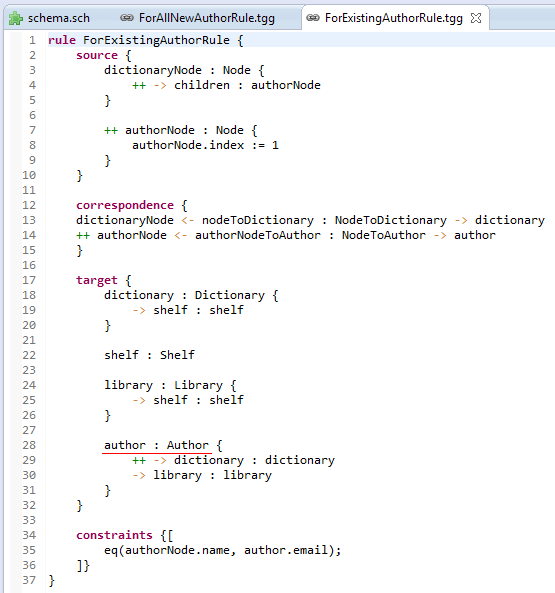
\includegraphics[width=\textwidth]{eclipse_ForExistingAuthorRule}
  \caption{ForExistingAuthor complete}
  \label{eclipse:ForExistingAuthorRule}
\end{center}
\end{figure}


\item[$\blacktriangleright$] Your final schema should now resemble..

\begin{figure}[htbp]
\begin{center}
  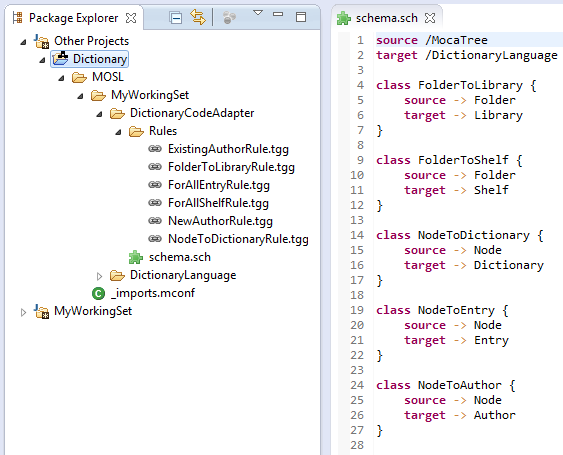
\includegraphics[width=\textwidth]{eclipse_finalSchema}
  \caption{Final schema}
  \label{eclipse:schemaFinal}
\end{center}
\end{figure}

\item[$\blacktriangleright$] Awesome work, dudes! Now build! If any errors form, be sure to double check your work for spelling or character typos. Else, Run
TGGMain by pressing the green button on the tool bar next to the funny-lookin' bug.

% New section to handle the multiple authors

\end{itemize}
